\clearpage
\section{Experiment Results}
在 Results 中,我想要討論我的 Best FID Score 的結果是如何獲得的,然後討論不同的 Inpainting 策略對於 FID Score 的影響,最後附上更多的修復圖片結果。


\subsection{The best FID score results}
由於我留給訓練的時間比較少,在這次長時間的訓練中,我使用的 batch size 是 64,learning rate 是 8e-5,訓練 300 個 epoch,這樣的訓練方式其實還沒有達到最好的效果,我們可以從下圖的 loss 並未開始反彈,以及我的最好的 checkpoint 是在最後一個 epoch 的時候的,所以我的 Best FID Score 的結果是 29.10 還有可以優化的空間。

在生成圖像的時候,我是使用 Linear 的 gamma 函數,總迭代數量為 12 ,然後取甜蜜點為第8次的迭代結果。

\begin{figure}[h]
    \centering
    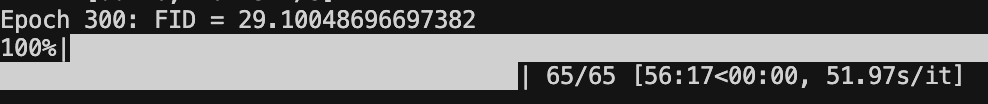
\includegraphics[width=\textwidth]{figures/best_fid_score.png}
    \caption{最佳 FID 分數結果}
    \label{fig:best_fid_score}
\end{figure}


\begin{figure}[h]
    \centering
    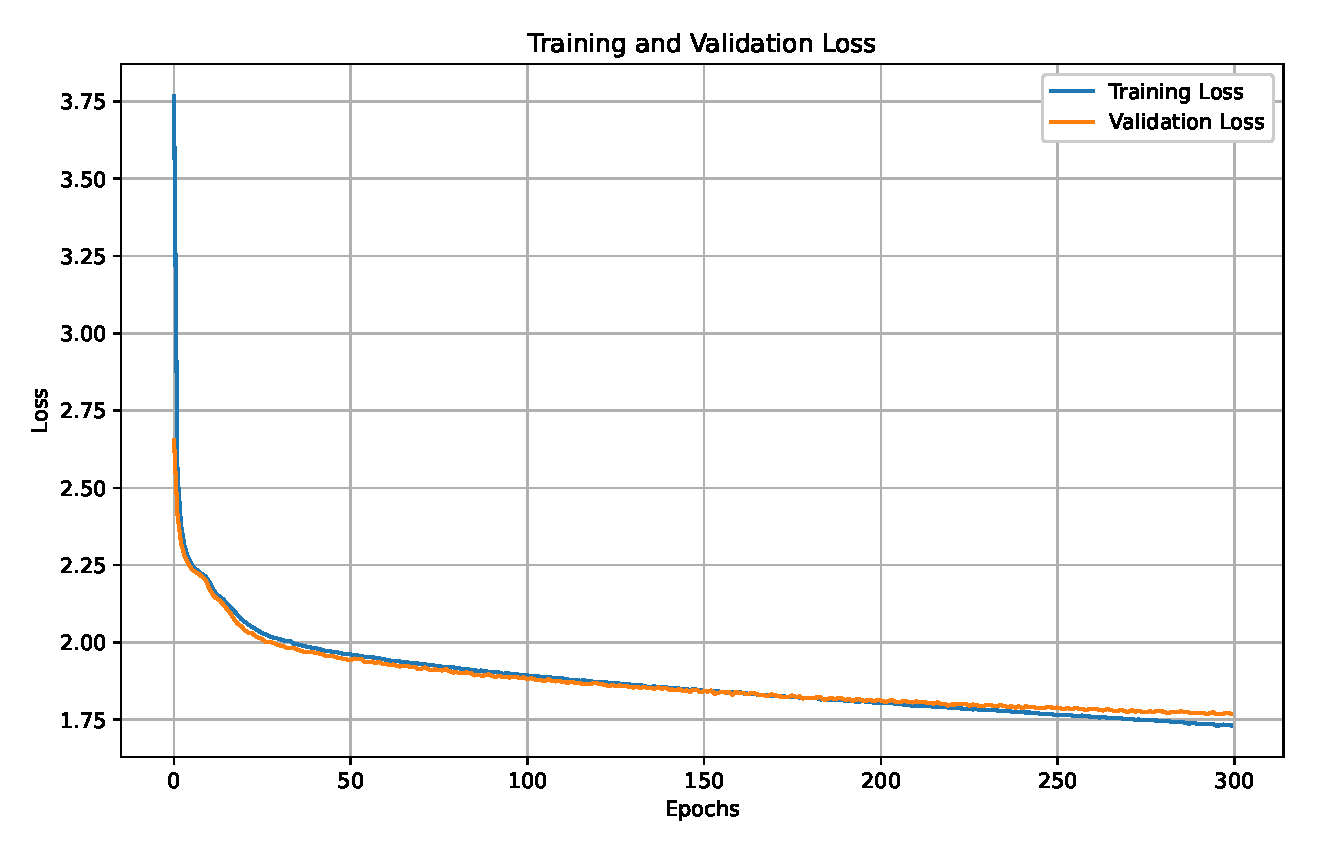
\includegraphics[width=\textwidth]{figures/loss_plot.eps}
    \caption{損失函數圖表}
    \label{fig:loss_plot}
\end{figure}

接著讓我們分析 Best FID Score 的結果。觀察生成過程,模型首先從左上角的缺陷開始填補,然後處理鼻子區域。值得注意的是,剩餘的缺陷主要是散佈在各個區域的小細節,這些細節通常是連接主要區域的部分。這種由主要區域到細節的填補策略非常符合直覺,因為它優先處理視覺上最顯著的部分,再逐步完善細節,使整體修復效果更加自然且連貫。

\begin{figure}[h]
    \centering
    \begin{subfigure}{\textwidth}
        \centering
        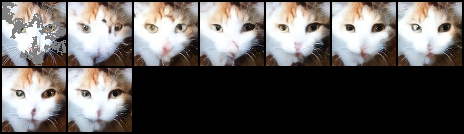
\includegraphics[width=0.8\textwidth]{figures/test_69.png}
        \label{fig:test_69}
    \end{subfigure}
    \vspace{1cm}
    \begin{subfigure}{\textwidth}
        \centering
        
\includegraphics[width=0.8\textwidth]{figures/mask_test_69.png}
        \label{fig:mask_test_69}
    \end{subfigure}
    \caption{測試圖像與其對應的遮罩示例。上方為原始圖像,下方為遮罩圖像。}
    \label{fig:test_and_mask}
\end{figure}






\clearpage
\subsection{Discussion on the Impact of Different Inpainting Strategies on FID Score}

由於畫出每個 epoch 的 FID Score 的圖表是個蠻大的計算量,所以我先使用 50 epoch 的結果來討論不同的 Inpainting 策略對於 FID Score 的影響。 在這裡我所有的迭代次數與取甜蜜點的策略都是相同的 12,以及一個 linear half 是代表 20 次迭代,然後甜蜜點設為 10。
我們可以看到 line half 的策略在 FID Score 上表現的最好,所以我們可以得到結論是需要使用甜蜜點設定讓模型提早退出,這樣可以讓模型有更好的表現,可是我沒有辦法做更詳細的測試,所以我使用助教提供的總迭代次數 12 的策略以及甜蜜點為 8 的策略來測試我的最長實驗,300 epoch 的結果。


\begin{figure}[h]
    \centering
    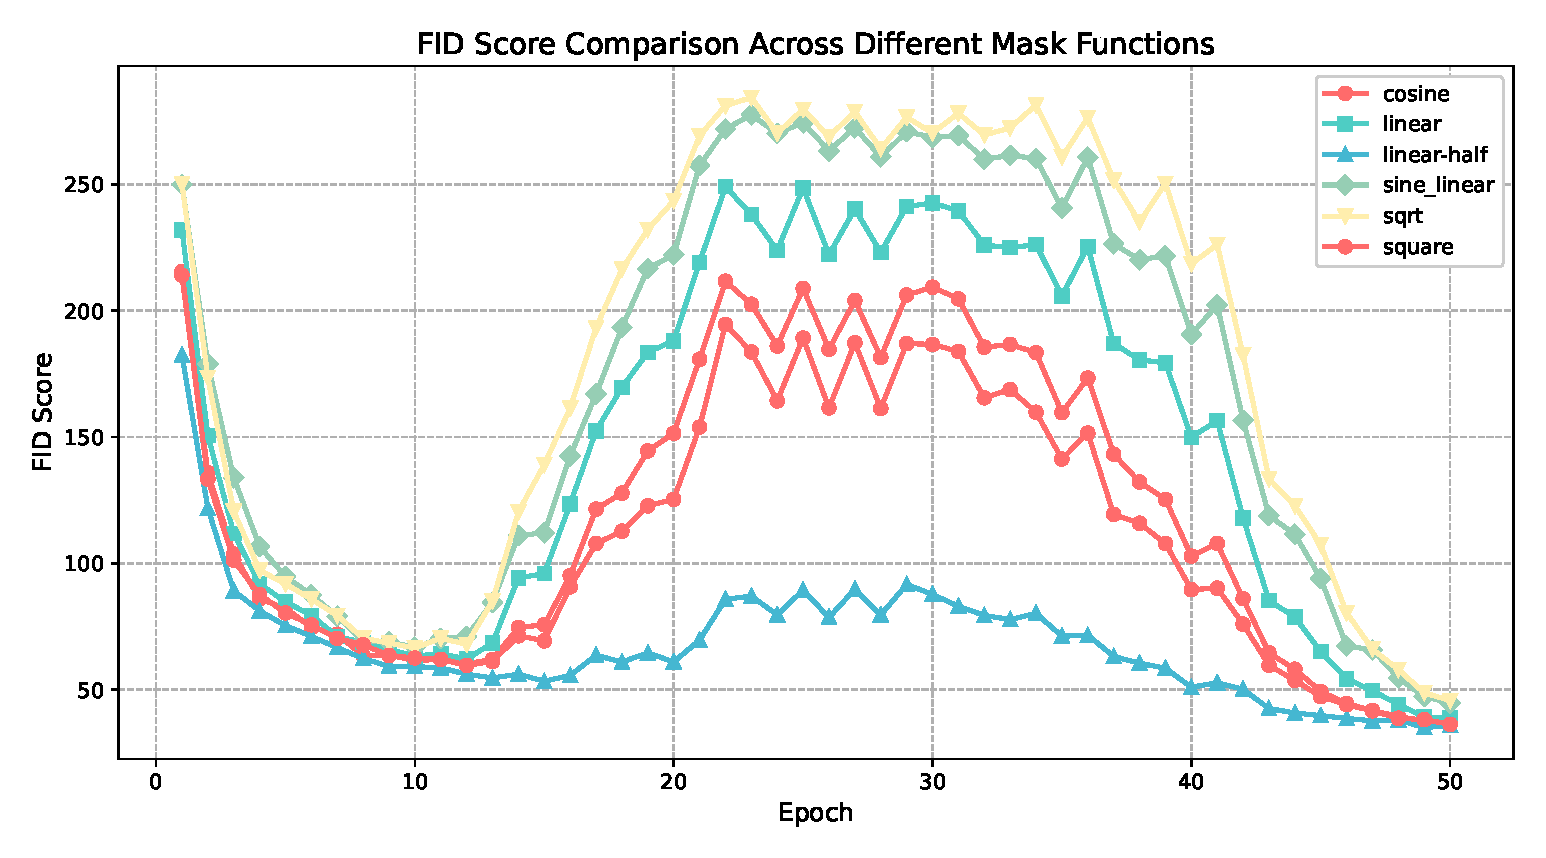
\includegraphics[width=\textwidth]{figures/fid_comparison.eps}
    \caption{不同策略的 FID 分數比較}
    \label{fig:fid_comparison}
\end{figure}



\clearpage
\begin{figure}[h]
    \centering
    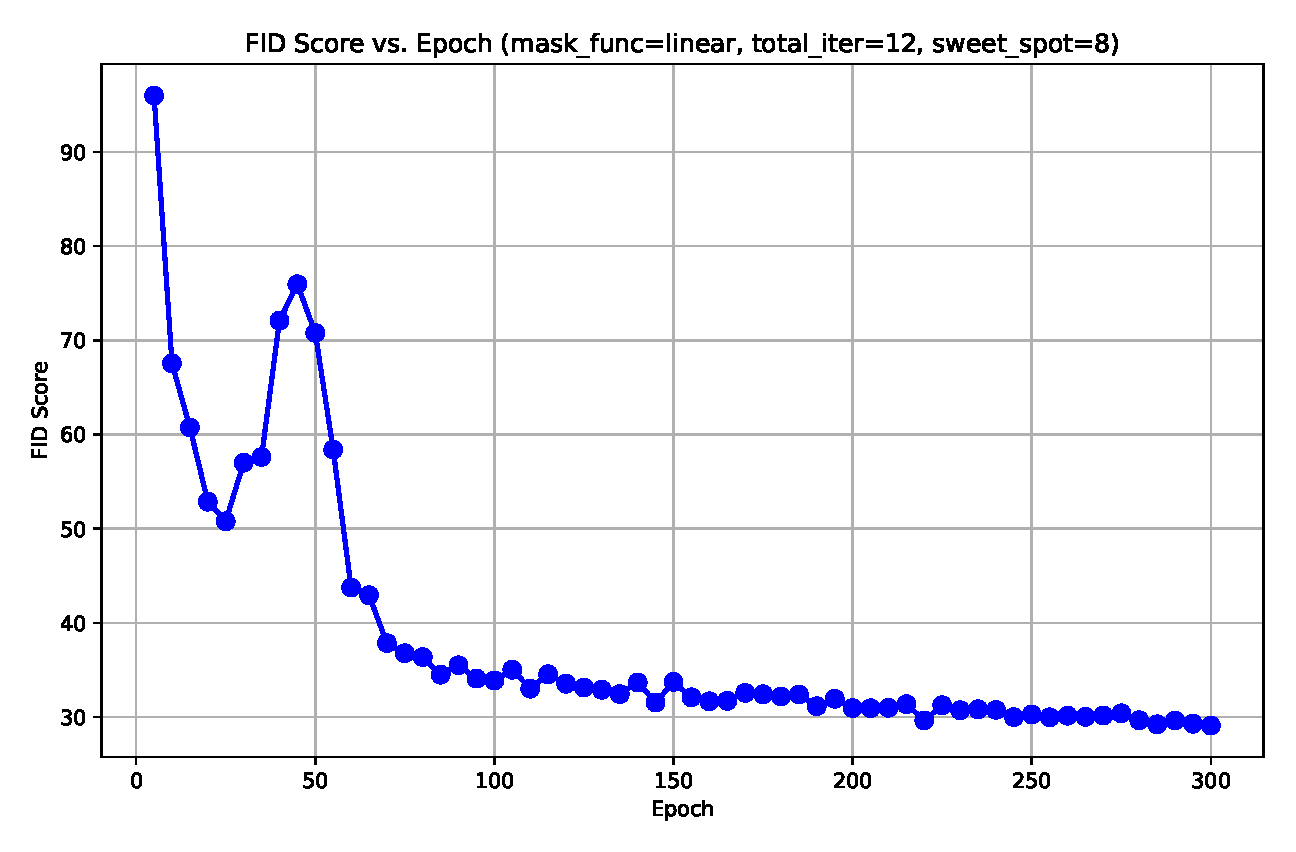
\includegraphics[height=7.5cm]{figures/fid_vs_epoch.eps}
    \caption{FID 分數隨訓練週期變化圖}
    \label{fig:fid_vs_epoch}
\end{figure}






\begin{figure}[h]
    \centering
    \begin{subfigure}{\textwidth}
        \centering
        
\includegraphics[width=0.8\textwidth]{figures/test_48.png}
        \label{fig:test_48}
    \end{subfigure}
    \vspace{1cm}
    \begin{subfigure}{\textwidth}
        \centering
        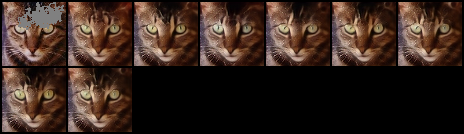
\includegraphics[width=0.8\textwidth]{figures/test_303.png}
        \label{fig:test_303}
    \end{subfigure}
    \caption{更多測試圖像示例。上方為測試圖像 48,下方為測試圖像 303。}
    \label{fig:test_examples}
\end{figure}


這裏可以看到 FID Score 還在下降,但是從更多測試圖像範例來看,效果其實已經不錯了。

最後我想說,這次的作業真的蠻有趣的,透過串接模型,來實現一個簡單的修復模型,尤其是在 code review 的時候,我覺得學到很多之前沒有學過的東西,而且是被驗證過的實用技巧。




